% úvod
Konečně se dostáváme k něčemu reálnému. Zde popíši hardwarovou část řešení tj. Co vlastně bude měřit, čím budu 
měřit\ldots

% měřící stanice
Možných základů pro měřící stanici, jednodeskových počítačů, je dnes na trhu mnoho od různých osmibitů, až po počítače 
na architektuře ARM,  které dosahují výkonu srovnatelného s mobilními telefony. Já jsem pro mé řešení zvolil Raspberry 
Pi ve verzi 2 a to z několika důvodů. Jednak ho mám k dispozici a dále mi nabízí běžící Linux a tudíž za mne řeší 
spoustu problémů, od síťové komunikace, po třeba synchronizaci času. Navíc mám k dispozici spoustu digitálních pinů pro 
připojení různých senzorů, též mám vyřešené i místní úložiště, data se mohou ukládat na SD kartu ze které běží celý 
systém a výrazně to zjednodušuje vývoj, poněvadž mohu nahrávat nové verze programů vzdáleně, a i vzdáleně sledovat 
jejich běh, což je pro mě výhodné, neb terárium nemám v pokoji, kde programuji. Samozřejmě že toto řešení má i své 
nevýhody. Například v případě, že bych chtěl měřit analogové hodnoty, bych musel dokupovat převodník z analogového 
signálu na digitální, či v případě nutnosti rozšíření na více míst, by to nebylo ekonomicky výhodné, přeci jen Raspberry 
Pi stojí kolem 1000 Kč. Nebo pokud bych chtěl zařízení napájet z akumulátoru, tak též s odběrem kolem půl ampéru to 
nebude to pravé ořechové. Avšak v případě zmíněných problémů mi zvolené celkové řešení umožňuje poměrně komfortně změnit 
základ stanice na něco vhodnějšího, za předpokladu, že se zvolená deska zvládne připojit na lokální síť. Například mohu 
použít oblíbenou desku ESP8266 či ESP32, které se cenově pohybují v řádu stokorun, pinů mají dostatek, disponují Wifi 
čipem a umožňují použití nízko odběrových módů při běhu na baterii.
\begin{figure}[H]
		\centering
    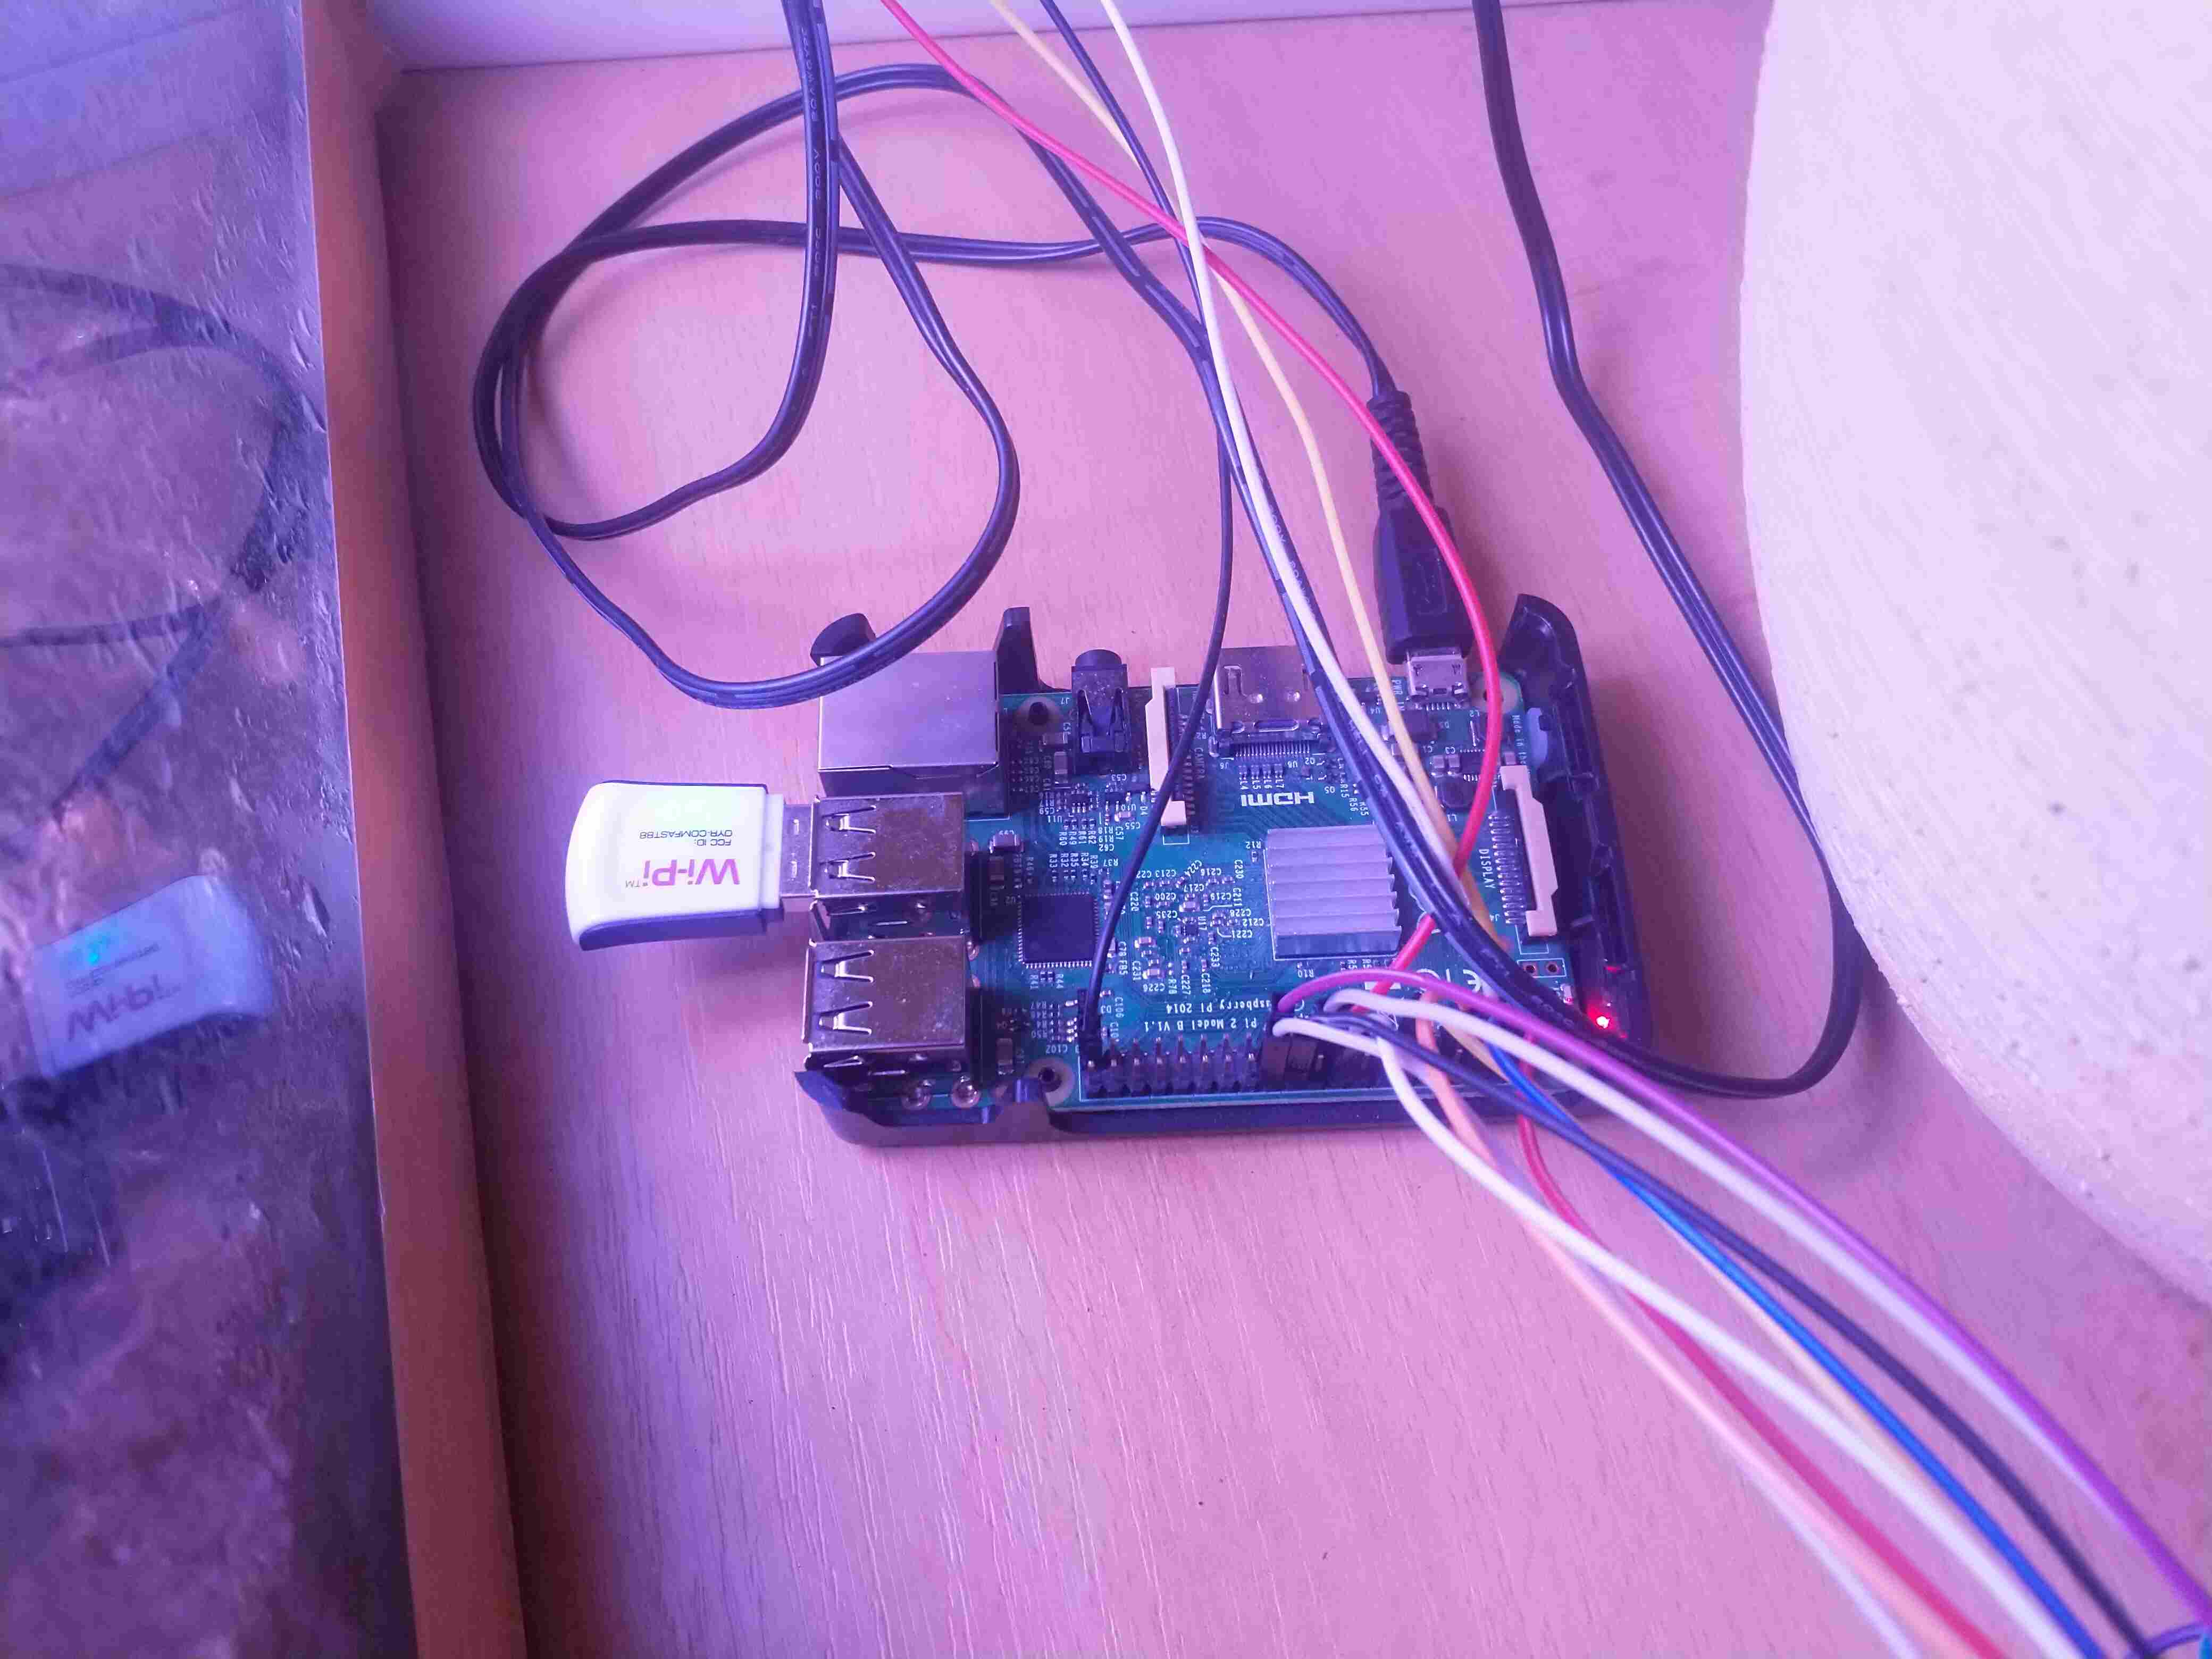
\includegraphics[width=\textwidth]{RPi2.jpg}
    \caption{Měřící stanice}
\end{figure}

% senzory
% BME280
A teď součást bez které by zbytek byl k ničemu, samotné senzory. Pro měření v samotném teráriu jsem zvolil BME280. Jedná 
se o senzor od firmy Bosh pro měření teploty, vlhkosti a atmosférického tlaku, vzhledem k tomu, že se dodává pouze v SMD 
variantě, jsem zvolil modul, který obsahuje tento senzor, potřebné součástky kolem a má vyvedenou I2C sběrnici, pro 
snadné připojení k řídící desce. Dal by se též použít libovolný jiný senzor obdobných parametrů, ale tento má příjemnou 
cenu a velmi dobrou přesnost měření, a navíc se díky I2C snadno propojí se zbytkem systému.
\begin{figure}[H]
		\centering
    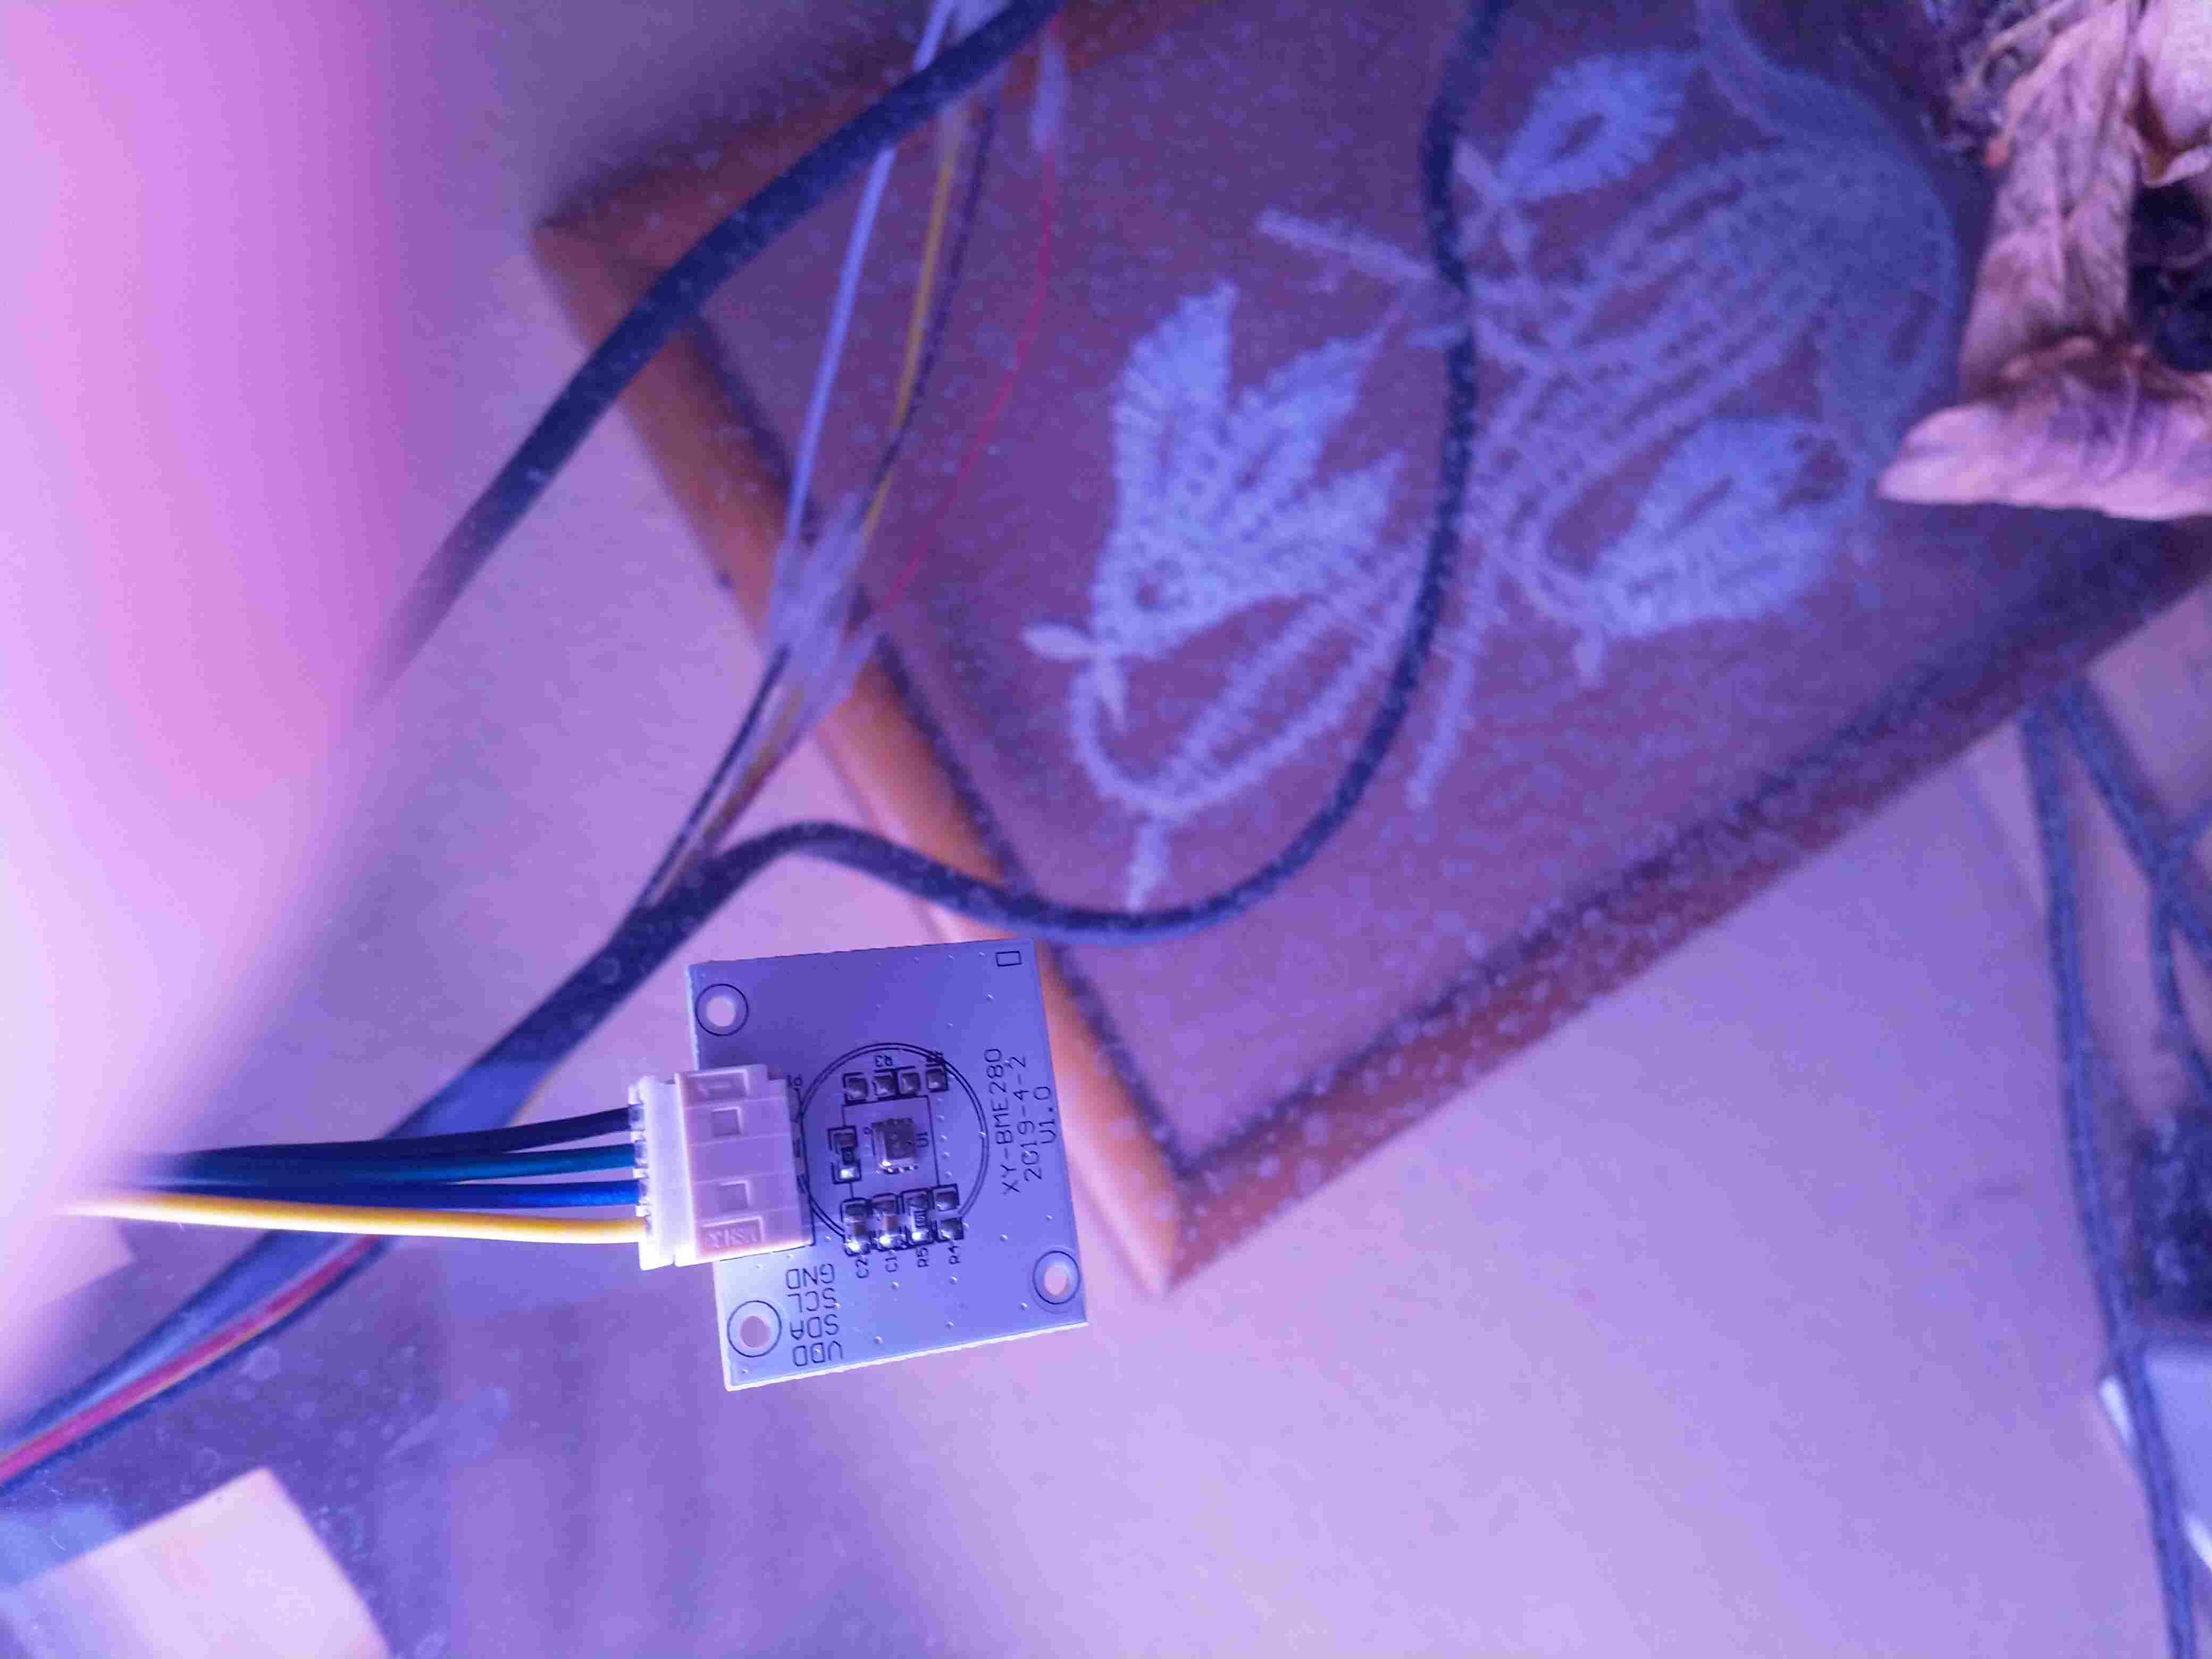
\includegraphics[angle=270,width=0.6\textwidth]{BME280.jpg}
    \caption{Modul s BME280, stříbrný čtvereček uprostřed}
\end{figure}

% DS1820
Za účelem případné další analýzy, jsem umístil pár senzorů i mimo terárium, abych mohl sledovat závislost teploty vně 
a uvnitř. Tady už nejde tolik o přesnost, takže jsem použil senzory co jsem našel doma. Na měření teploty jsem použil 
senzor od firmy DS1820. Jde o jednoduché a levné čidlo, moje je v pouzdru TO-92, to se používá třeba taky pro 
tranzistory, OneWire sběrnicí, speciální sběrnice od firmy Dallas, která potřebuje pouze tři dráty a umožňuje i použití 
pouze dvou a digitálním měřením teploty s přesností 0.5 \textdegree C.
\begin{figure}[H]
		\centering
    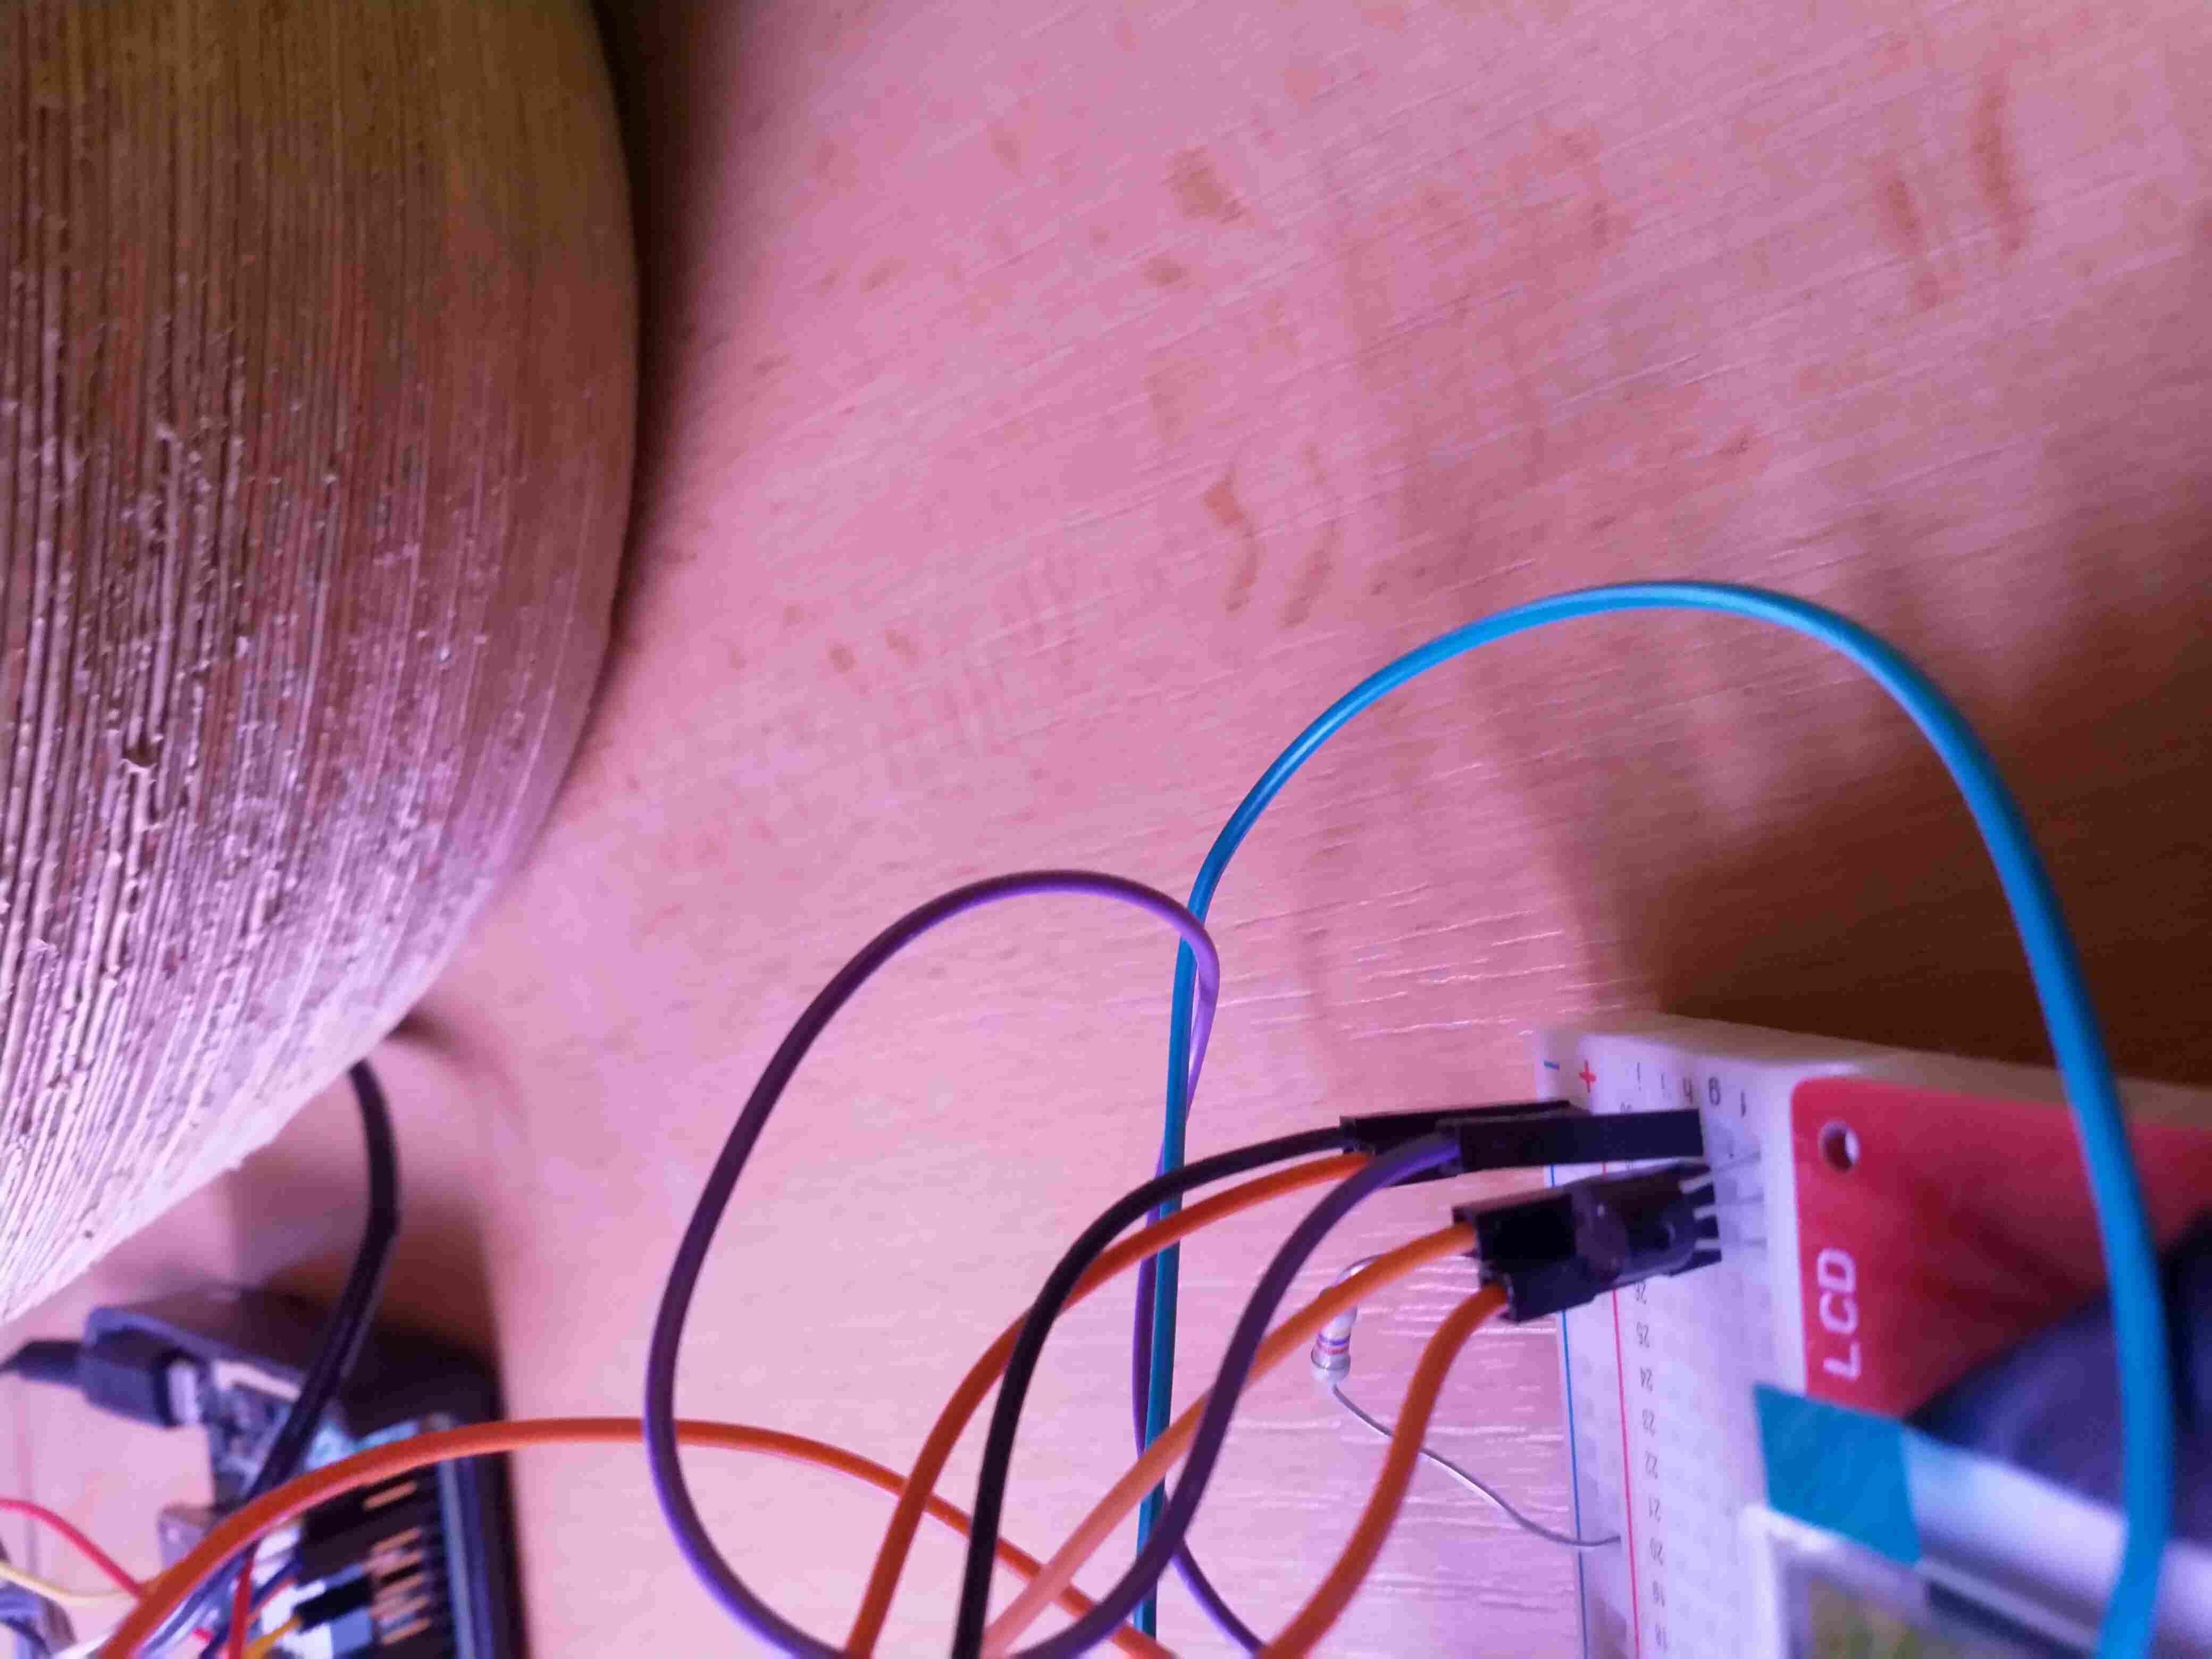
\includegraphics[angle=270,width=0.6\textwidth]{DS1820.jpg}
    \caption{DS1820}
\end{figure}

% DHT11
A jako poslední jsem použil oblíbené čidlo teploty a vlhkosti DHT11. Jde o čínský výrobek v modré krabičce se čtyřmi 
vývody, z nichž jeden je neaktivní. Čidlo používá vlastní sběrnici, které však též stačí tři dráty, jako výše zmíněné 
OneWire. Senzor teploty jsem zdvojit, poněvadž toto čidlo je velmi levné a bohužel též nepřesné, rozlišení 1 \textdegree C při 
možné odchylce až 2 \textdegree C, není úplně ideální, proto jsem ho doplnil výše zmíněným teploměrem. U vlhkosti je to podobné, 
ale vzhledem k tomu, že se jednak hůře ovlivňuje a také se pohybuje ve větším intervalu než teplota mi odchylka 5 \% zas 
tolik nevadí.
\begin{figure}[H]
		\centering
    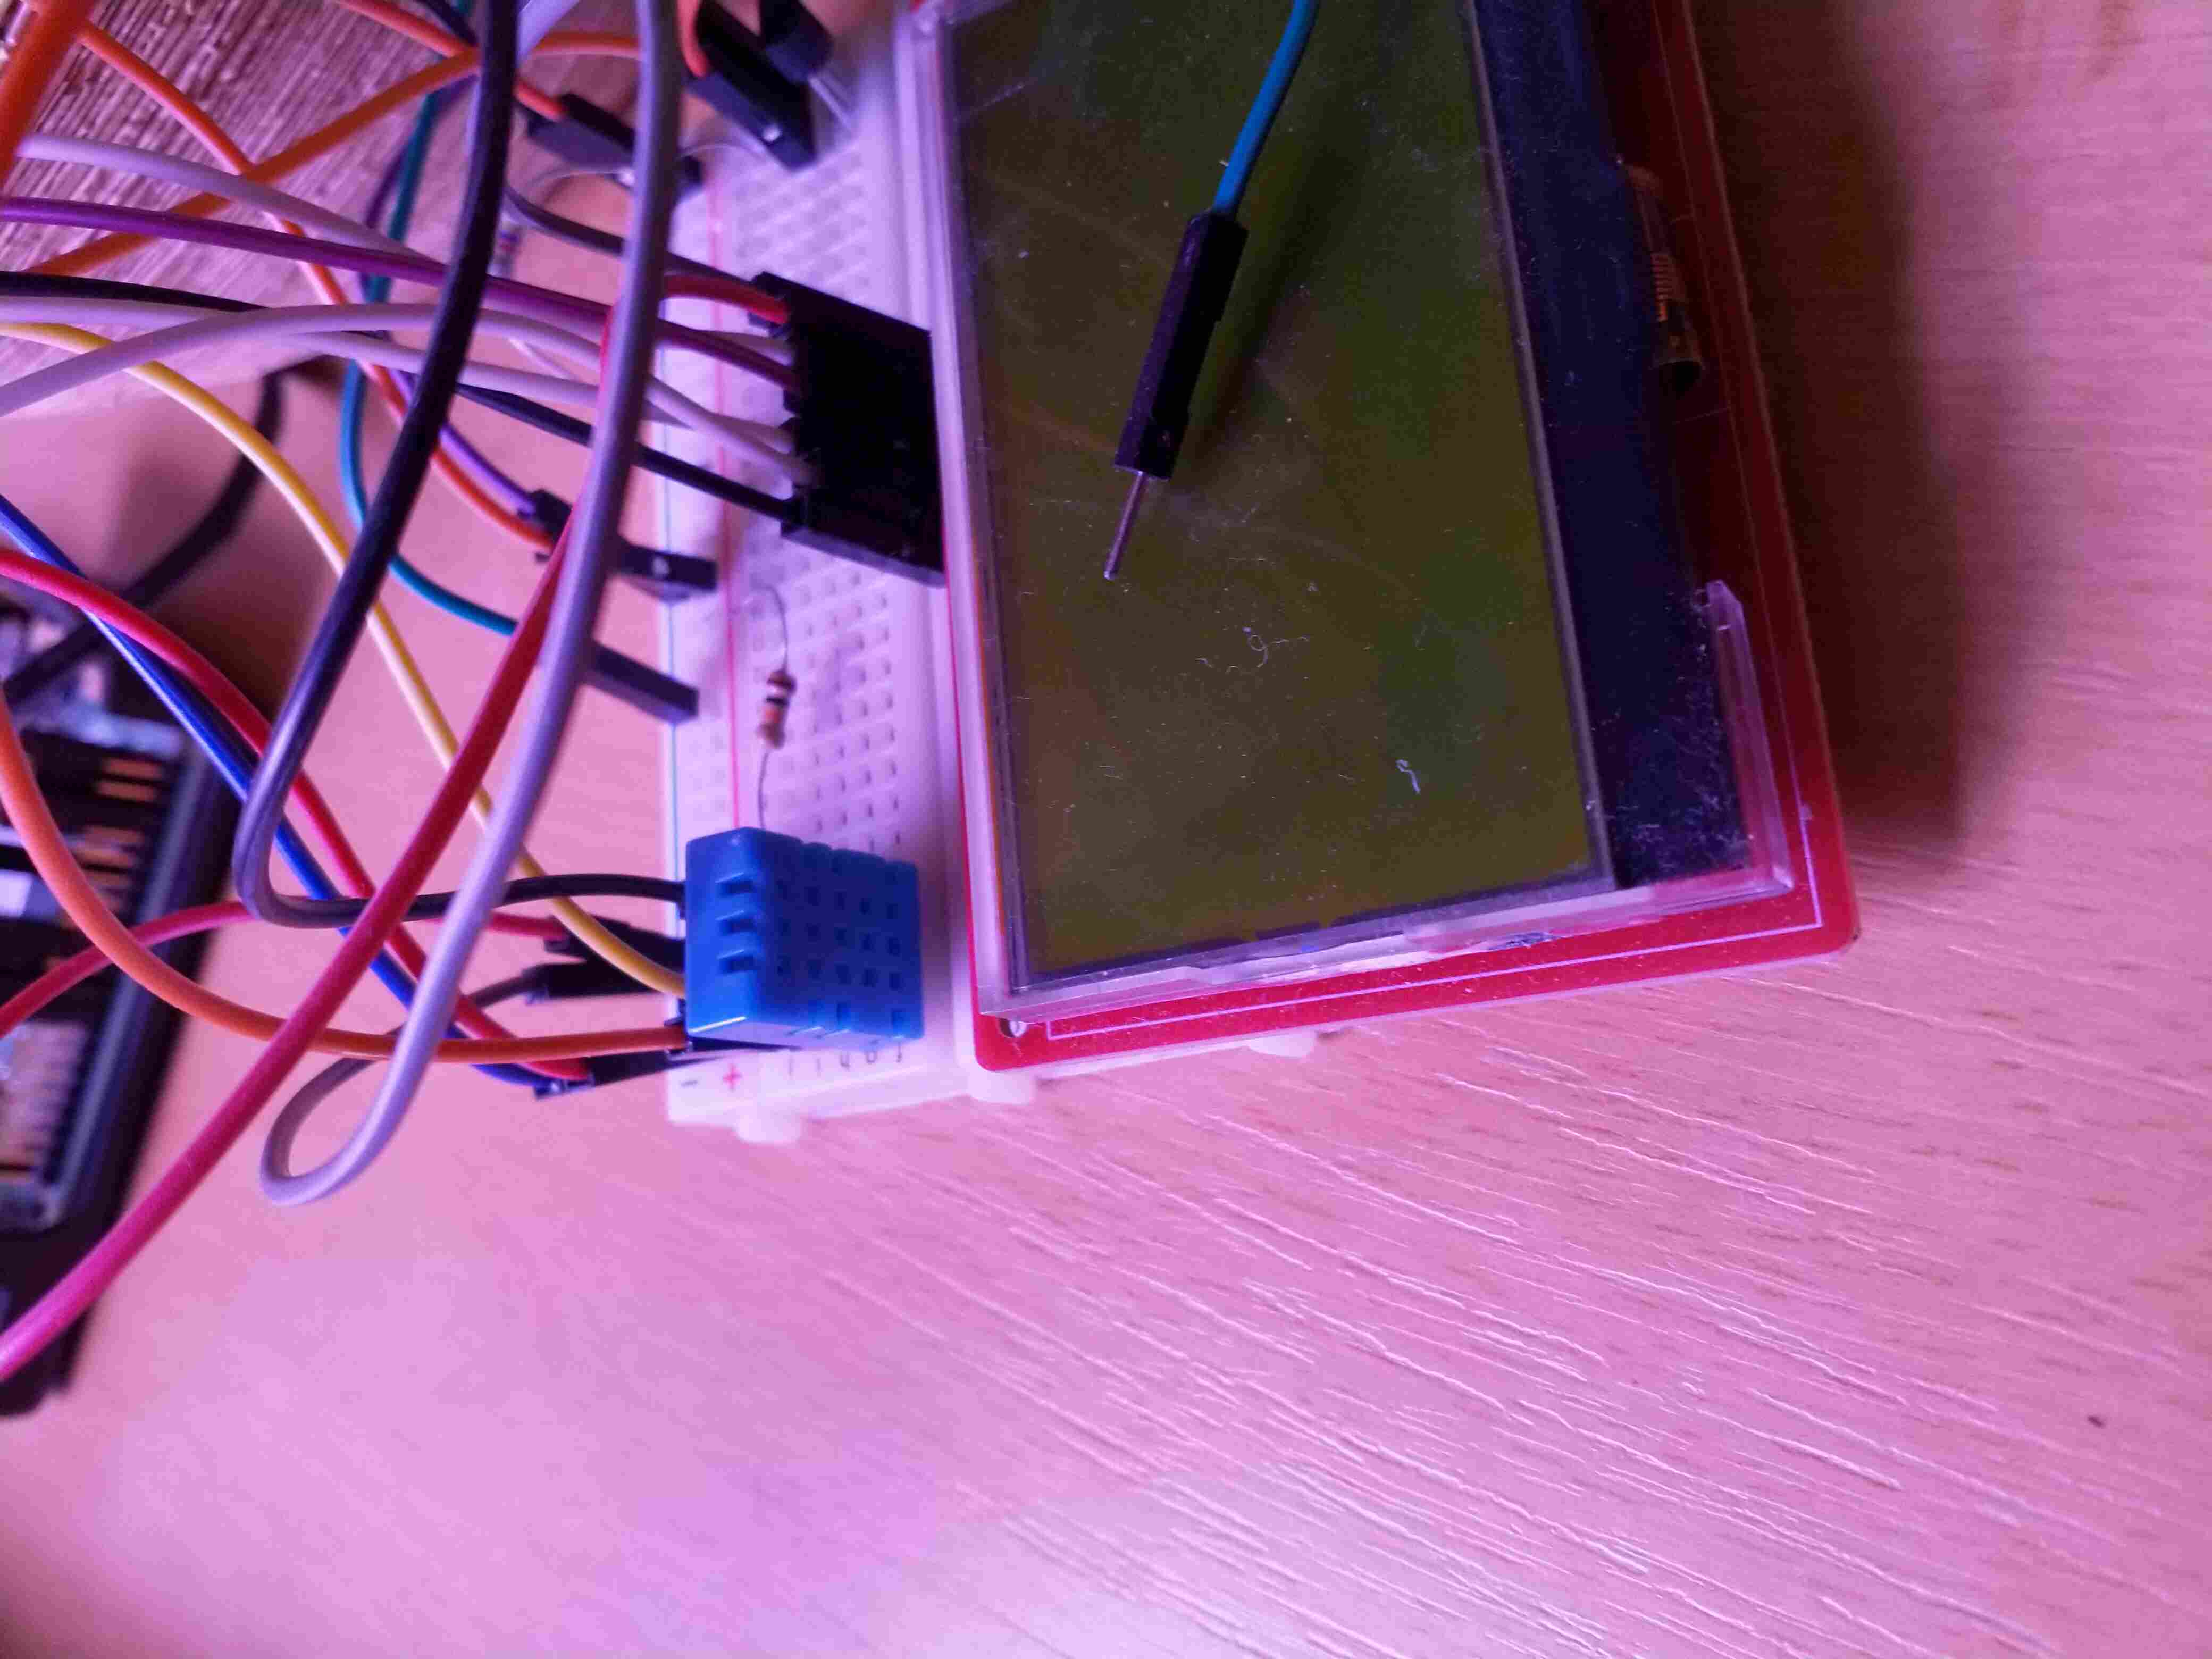
\includegraphics[angle=270,width=0.6\textwidth]{DHT11.jpg}
    \caption{DHT11}
\end{figure}

% gateway
Jako brána pro komunikaci s internetem se dá taky použit téměř cokoli, ale přeci jen jsou na ní kladeny větší nároky než 
na měřící stanici. Mimo nutnosti možnosti připojení do sítě je též třeba výpočetní výkon a paměť, dostatečná na 
komunikaci s cloudem, řešení šifrování, běh nějakého message brokera\ldots, tedy nejlépe nějakou desku s operačním 
systémem, který mi tohle všechno umožní. Já jsem zvolil opět Raspberry Pi, tentokrát ve verzi 3 opět z velmi 
jednoduchého důvodu, už mi doma běží, jako takový domácí server.
